% Nome del file: ManualeUtente.tex
% Percorso: \gl{template}
% Autore: Vault-Tech
% Data creazione: 10.05.2016
% E-mail: vaulttech.swe@gmail.comcom
%
% Diario delle modifiche: interno al file.

\documentclass[a4paper, titlepage]{article}

\usepackage[margin=3cm]{geometry}
\usepackage{../../Stile}
\usepackage{../../Comandi}

\setcounter{secnumdepth}{5}
\setcounter{tocdepth}{5}

\def\NOME{Manuale Utente}
\def\VERSIONE{1.0}
\def\DATA{04.04.2016}
\def\REDATTORE{Michela De Bortoli \\ & Filippo Tesser}
\def\VERIFICATORE{Simone Boccato \\ & Miki Violetto}
\def\RESPONSABILE{Giacomo Beltrame}
\def\USO{Esterno}
\def\DISTRIBUZIONE{\COMMITTENTE \\ & \CARDIN \\ & \PROPONENTE}


\begin{document}
	
	\pagestyle{fancy}	
	\pagenumbering{Roman}
	\rfoot{Pagina \thepage{} di \pageref{lastromanpage}}
	
	\maketitle
	
	\begin{diario}
	\recap{Approvazione del documento}{Michela De Bortoli}{Responsabile}{06.04.2016}{3.0}
	\recap{Correzione errori individuati}{Michela De Bortoli}{Analista}{06.04.2016}{2.10}
	\recap{Verifica dell'intero documento}{Rudy Berton}{Verificatore}{05.04.2016}{2.9}
	\recap{Stesura appendice D}{Giacomo Beltrame}{Analista}{04.04.2016}{2.8}
	\recap{Verifica appendici A e B}{Giacomo Beltrame}{Verificatore}{03.04.2016}{2.7}
	\recap{Stesura test di integrazione}{Rudy Berton}{Amministratore}{02.04.2016}{2.6}
	\recap{Stesura test di sistema}{Vassilikì Menarin}{Progettista}{02.04.2016}{2.5}
	\recap{Modifica della sezione A.3.3 dell'appendice}{Filippo Tesser}{Analista}{01.04.2016}{2.4}
	\recap{Incremento test di accettazione}{Michela De Bortoli}{Progettista}{01.04.2016}{2.3}
	\recap{Inizio stesura specifica dei test (appendice B)}{Michela De Bortoli}{Progettista}{31.03.2016}{2.2}
	\recap{Incremento dell'appendice A}{Filippo Tesser}{Analista}{31.03.2016}{2.1}
	\recap{Approvazione documento}{Miki Violetto}{Responsabile}{23.02.2016}{2.0}
	\recap{Verifica delle sezioni modificate}{Rudy Berton}{Verificatore}{22.02.2016}{1.2}
	\recap{Revisione correttiva dei contenuti rispetto alle segnalazioni del committente}{Giacomo Beltrame}{Analista}{20.02.2016}{1.1}
	\recap{Approvazione documento}{Vassilikì Menarin}{Responsabile}{20.01.2016}{1.0}
	\recap{Verifica del documento}{Simone Boccato}{Verificatore}{19.01.2016}{0.9}
	\recap{Stesura appendice D}{Rudy Berton}{Analista}{18.01.2016}{0.8}
	\recap{Correzione errori segnalati}{Rudy Berton}{Analista}{16.01.2016}{0.7}
	\recap{Verifica del documento}{Filippo Tesser}{Verificatore}{15.01.2016}{0.6}
	\recap{Stesura appendici A, B e C}{Rudy Berton}{Analista}{11.01.2016}{0.5}
	\recap{Fine stesura Gestione della qualità e stesura sezione Gestione amministrativa della revisione}{Rudy Berton}{Analista}{08.01.2016}{0.4}
	\recap{Inizio stesura Gestione della qualità}{Rudy Berton}{Analista}{05.01.2016}{0.3}
	\recap{Stesura sezione Obiettivi di qualità}{Rudy Berton}{Analista}{03.01.2016}{0.2}
	\recap{Stesura sezione Introduzione}{Rudy Berton}{Analista}{02.01.2016}{0.1}
\end{diario}
	
	\newpage
	\tableofcontents
	\newpage
	\listoffigures
	\newpage
	\listoftables\label{lastromanpage}
	
	\newpage
	\clearpage	
	\pagenumbering{arabic}
	\rfoot{Pagina \thepage{} di \pageref*{LastPage}}
	%Deve esserci per permettere i riferimenti incrociati di colore blu
	\hypersetup{linkcolor=blue}
	
	\section{Introduzione}
	\subsection{Scopo del documento}
	Questo documento ha lo scopo di fornire un aiuto all'utente che si trovi ad utilizzare il software
	Quizzipedia per le prime volte illustrandone il funzionamento di base dello stesso.
	
	\subsection{Scopo del prodotto}
	\SCOPO
	
	\subsection{Riferimenti}	
	\subsubsection{Riferimenti normativi}
	\begin{itemize}
		\item \bold{\gl{Capitolato} d'appalto C5:} Quizzipedia: \gl{software} per la gestione di questionari \newline \url{http://www.math.unipd.it/~tullio/IS-1/2015/Progetto/C5.pdf};
		\item \bold {Norme di progetto:} \NdPdoc.
	\end{itemize}
	\newpage
	
	\section{Homepage}
	
	\subsection{Registrazione}
	\begin{figure}[!ht]
		\centering
		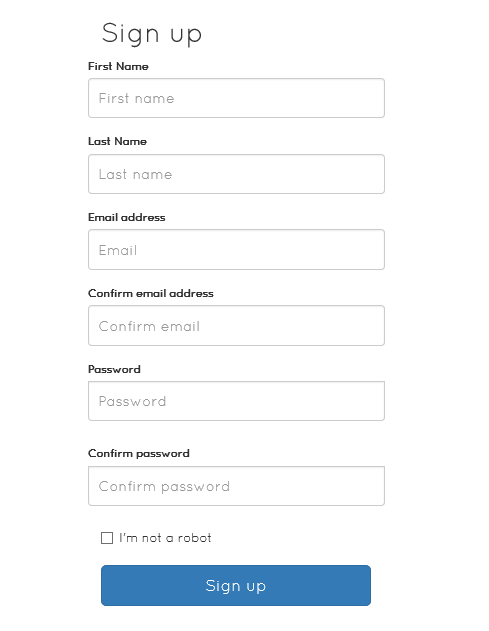
\includegraphics[scale=1]{Img/register.png}
		\caption{Schermata di registrazione}
	\end{figure}
	Selezionare la voce 'Register' in alto a destra nella barra di navigazione porta alla pagina di registrazione.
	Per completare la registrazione è necessario inserire nell'apposito form:
	\begin{itemize}
		\item nome,
		\item cognome,
		\item indirizzo email,
		\item conferma dell'indirizzo email,
		\item password,
		\item conferma della password.
	\end{itemize}
	Se i dati sono stati inseriti correttamente, una volta effettuata la conferma cliccando sul pulsante 'Conferma', la registrazione sarà completata con successo.
	Verrà visualizzato un messaggio di errore nel caso le seguenti condizioni non siano verificate:
	\begin{itemize}
		\item l'indirizzo email immesso non deve essere associato a un account già esistente;
		\item l'indirizzo email deve avere un formato valido;
		\item la password immessa deve essere valida: compresa fra i 8 e i 16 caratteri;
		\item la password immessa e la sua conferma devono coincidere;
		\item tutti i campi devono essere riempiti.
	\end{itemize}
	
	\subsection{Autenticazione}
	\begin{figure}[!ht]
		\centering
		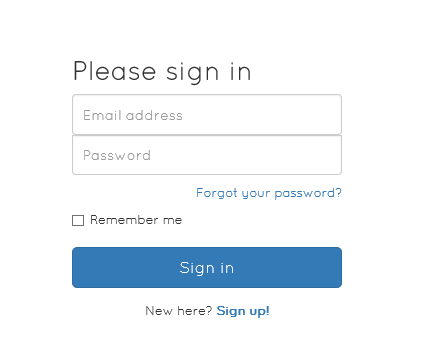
\includegraphics[scale=1]{Img/login.png}
		\caption{Schermata di autenticazione}
	\end{figure}
	Selezionare la voce 'Login' in alto a destra nella barra di navigazione per effettuare l'accesso al sistema. Per autenticarsi sarà necessario immettere il proprio indirizzo email e la password corrispondente. Se l'indirizzo email corrisponde a un account registrato e la password inserita è corretta, l'autenticazione sarà completata con successo.

	\subsection{Recupero password}
	Nel caso l'utente non ricordi la propria password, è possibile ottenerne una temporanea compilando l'apposito form. Una volta inserito il proprio indirizzo email e confermata la richiesta, l'utente riceverà nell'indirizzo email fornito una password temporanea che potrà utilizzare nel prossimo accesso. È suggerito modificare la propria password dopo aver effettuato il recupero.
	
	\subsection{Ricerca enti e classi}
	
	
	\section{Quiz}
	
	\subsection{Ricerca quiz}
	 È possibile effettuare ricerche di quiz selezionando l'opzione 'Ricerca' nella barra di navigazione. La ricerca è personalizzabile attraverso diversi parametri:
	 \begin{itemize}
	 	\item materia,
	 	\item livello di difficoltà,
	 	\item parole chiave,
	 	\item etcc.
	 \end{itemize}
	 
	 \subsection{Svolgimento quiz}
	 
	 
	 \section{Utente autenticato}
	 
	 \subsection{Homepage}
	 
	 \subsection{Gestione profilo}
	
	 \subsection{Cambio password}
	 
	 
	 \section{Studente}
	 
	 \subsection{Ricerca quiz privati}
	 
	 \subsection{Visualizza storico dei quiz}
	 
	 
	 \section{Docente}
	 
	 \subsection{Gestione classe}
	 
	 \subsection{Gestione quiz}
	 
	 \subsection{Gestione domande}
	 
	 \subsection{Visualizza statistiche}
	 
	 
	 \section{Responsabile}
	 
	 \subsection{Gestione argomento}
	 
	 \subsection{Creazione argomento}
	 
	 \subsection{Rimozione utenti}
	 
	 \subsection{Gestione enti e classi}
	 
	
\end{document}